\documentclass[11pt,a4paper]{article}
\usepackage[utf8]{inputenc}
\usepackage[T1]{fontenc}
\IfFileExists{french.ldf}{\usepackage[french]{babel}}{\usepackage[english]{babel}}% français sur Overleaf
\usepackage{lmodern,microtype}
\usepackage[margin=2.5cm]{geometry}
\usepackage{booktabs,array,graphicx,xcolor}
\usepackage{tikz}
\usetikzlibrary{calc,arrows.meta,positioning}
\usepackage[round,authoryear]{natbib}
\usepackage[hidelinks]{hyperref}
\usepackage{setspace}\onehalfspacing
\newcommand{\aremplir}[1]{\textbf{\textcolor{red}{[À remplir : #1]}}}

\title{Chercher ou répondre ?\\ Agents de recherche entraînés par renforcement et harnais fixes :\\ une comparaison à corpus et questions identiques}
\author{Valentin Proux}
\date{Version de travail du 3 novembre 2026}

\begin{document}
\maketitle

\begin{abstract}
\noindent\textbf{Contexte.} Pour répondre à des questions factuelles, un modèle de langage peut utiliser un moteur de recherche, soit dans un schéma fixé par le programmeur (RAG, ReAct, IRCoT), soit en ayant appris par renforcement à décider seul quand et quoi chercher (Search-R1).
\textbf{Lacune.} Les comparaisons publiées sont le plus souvent faites par les auteurs de chaque méthode, avec leurs propres lignes de base.
\textbf{Méthode.} Nous comparons six systèmes construits sur la même famille de modèles (Qwen2.5, 3 milliards de paramètres), avec le même corpus, le même retriever et les mêmes questions, sur un jeu vu à l'entraînement (Natural Questions) et un jeu non vu (TriviaQA).
\textbf{Résultats.} \aremplir{résultats chiffrés, à écrire après les runs}
\textbf{Apport.} \aremplir{une phrase sur ce que l'on retient, à écrire après les runs}
\medskip

\noindent\textbf{Mots-clés :} agents de recherche, apprentissage par renforcement, génération augmentée par la recherche, petits modèles de langage.
\end{abstract}

\section{Introduction}

Un modèle de langage ne sait pas tout, et ne sait pas toujours ce qu'il ne sait pas. Pour répondre à une question factuelle rare, récente ou composée de plusieurs étapes, on lui donne un moteur de recherche. Reste à décider quand l'appeler et avec quelle requête.

Deux familles de solutions coexistent. Dans la première, le \emph{harnais} est fixé par le programmeur : on cherche toujours une fois avant de répondre \citep{lewis2020retrieval}, ou l'on fait alterner pensée, action et observation guidées par un prompt \citep{yao2022react}, ou l'on cherche après chaque phrase de raisonnement \citep{trivedi2022interleaving}. Dans la seconde, le modèle \emph{apprend}, par une récompense portant sur la réponse finale, quand et quoi chercher : c'est le cas de Search-R1 \citep{jin2025search}, de R1-Searcher \citep{song2025r1} et de ReSearch \citep{chen2025research}. Les auteurs de Search-R1 rapportent, avec Qwen2.5-3B, un gain de 20~\% sur diverses lignes de base RAG « dans le même cadre » \citep{jin2025search}.

Ces comparaisons posent un problème de lecture : chaque équipe choisit ses lignes de base, souvent sur les jeux de questions utilisés à l'entraînement. \citet{zhao2026retrieval} font le même constat pour les méthodes d'entraînement : la croissance des méthodes a dépassé celle des comparaisons contrôlées. Dans le corpus que nous avons réuni (titres et résumés examinés, textes non lus en entier), nous n'avons pas repéré de comparaison contrôlée d'un agent entraîné avec les trois harnais fixes usuels, à corpus, retriever et questions identiques. Cette absence vaut pour notre recherche : elle ne prouve pas qu'une telle étude n'existe pas. Notre question est donc la suivante : \emph{à corpus et questions identiques, un agent de recherche entraîné par renforcement décide-t-il mieux quand et quoi chercher qu'un harnais fixe, et à quel coût ?}

Cet article présente la partie de cette étude que nous avons pu mener à petite échelle : six systèmes, deux jeux de questions, 100 questions par jeu. Il pose le cadre complet (section~\ref{sec:cadre} à~\ref{sec:hyp}) puis teste deux des quatre hypothèses de notre projet de mémoire. Les deux autres (effet d'une pénalité par recherche, effet d'un changement de retriever) sont présentées comme prolongements. La section~\ref{sec:revue} fait le point sur la littérature, la section~\ref{sec:methode} décrit le protocole, la section~\ref{sec:resultats} donne les résultats, et la section~\ref{sec:discussion} les discute.

\section{Revue de la littérature}\label{sec:revue}

\subsection{Démarche}
Cette revue est narrative. La recherche documentaire a utilisé OpenAlex et Consensus par l'intermédiaire d'un agent d'IA, le 3 novembre 2026. L'équation retenue croise le renforcement, la recherche agentique, la tâche de questions-réponses et les modèles de langage, depuis 2023 ; elle a renvoyé 103 résultats à la première exécution et 116 après sa réécriture à partir du journal, le même jour. Sur cinq articles témoins, elle ne retrouve que Search-R1 : ReAct, IRCoT et Self-RAG ne relèvent pas du renforcement, et le résumé de R1-Searcher n'emploie ni « search engine » ni « question answering ». Ces articles viennent donc de la première collecte thématique. Le détail des requêtes figure en annexe du carnet de bord. Les textes n'ont pas été lus en entier : ce que nous rapportons des études récentes vient de leur résumé.

\subsection{Harnais fixes}
La génération augmentée par la recherche (RAG) combine la mémoire du modèle et un index de documents \citep{lewis2020retrieval}. Ses variantes itératives ajoutent des recherches en cours de raisonnement : ReAct fait alterner raisonnement et actions d'outil \citep{yao2022react}, IRCoT entrelace recherche et chaîne de pensée \citep{trivedi2022interleaving}. D'autres travaux apprennent à décider \emph{si} il faut chercher, par un classifieur de complexité de la question \citep{jeong2024adaptive}, par l'incertitude de la génération \citep{jiang2023active,moskvoretskii2025adaptive} ou par la réflexion du modèle sur lui-même \citep{asai2023self}. Cette littérature part d'un constat : chercher n'aide pas toujours, et l'intérêt de la recherche dépend de ce que le modèle sait déjà \citep{mallen2022when,yin2023do}.

\subsection{Agents de recherche entraînés par renforcement}
Search-R1 entraîne un modèle à produire des requêtes pendant son raisonnement, avec une récompense simple fondée sur la justesse de la réponse finale \citep{jin2025search}. R1-Searcher \citep{song2025r1}, ReSearch \citep{chen2025research} et DeepResearcher \citep{zheng2025deepresearcher} suivent la même idée avec des variantes de récompense, de données ou d'environnement ; ZeroSearch remplace le moteur réel par un moteur simulé \citep{sun2025zerosearch}. Ces travaux s'appuient sur les algorithmes PPO \citep{schulman2017proximal} et GRPO \citep{shao2024deepseekmath}, popularisés pour le raisonnement par DeepSeek-R1 \citep{deepseekai2025deepseek}. Une étude empirique des auteurs de Search-R1 conclut que les récompenses de format sont utiles, que les récompenses intermédiaires sur la recherche ont peu d'effet, et que le choix du moteur de recherche pèse sur la dynamique de l'entraînement et sur la robustesse de l'agent \citep{jin2025empirical}. Une synthèse récente organise ce champ \citep{lin2025comprehensive}.

\subsection{Coût des recherches}
Plusieurs travaux traitent les appels comme un coût. Wang et al. cherchent à réduire les actions inutiles d'un agent \citep{wang2025acting}. ParallelSearch décompose les questions pour lancer les recherches en parallèle, ce qui réduit le nombre d'appels au modèle \citep{zhao2025parallelsearch}. AI-SearchPlanner optimise conjointement l'utilité et le coût de la planification \citep{mei2025ai}, et AdaSearch cherche l'équilibre entre connaissances du modèle et recherche \citep{lin2025adasearch}. La surrecherche est désormais définie et mesurée : \citet{wu2025search} rapportent qu'un modèle aurait pu éviter 27,7~\% de ses étapes de recherche, et SAAS la traite par une pénalité dans la récompense \citep{tang2026saas}. \citet{pezzuti2026how} publient environ un million de traces d'agents et observent des chaînes allant jusqu'à 186 appels pour une seule requête, dans un banc d'essai contrôlé.

\subsection{Retriever et bruit}
Le retriever compte : BM25 \citep{robertson2009probabilistic} est lexical, E5 \citep{wang2022text} est dense ; Search-R1 est entraîné avec E5. Des modèles se laissent distraire par des passages non pertinents \citep{yoran2023making} ou ignorent les informations placées au milieu d'un long contexte \citep{liu2023lost}. Ces effets limitent ce que l'on peut attendre d'une recherche réussie. \citet{zhao2026retrieval} signalent en outre un défaut de couverture du corpus Wikipédia 2018, dont la correction apporte plus que l'écart entre algorithmes d'entraînement : ce résultat, tiré du résumé, rend d'autant plus nécessaire notre mesure de couverture (section~\ref{sec:methode}).

\subsection{Lacune}
Les articles ci-dessus évaluent souvent leur méthode contre des lignes de base choisies par leurs auteurs. Trois travaux s'approchent de notre question. \citet{zhao2026retrieval} comparent de façon contrôlée des méthodes d'entraînement entre elles, et non des agents entraînés à des harnais fixes. \citet{raikote2026policy} oppose un contrôleur appris à des règles fixes, mais avec un modèle gelé. s3 entraîne un chercheur séparé contre le RAG naïf \citep{jiang2025s3}. La question de savoir si le gain vient de l'\emph{apprentissage de la décision de chercher} ou d'autres différences (modèle, prompt, retriever, jeux vus à l'entraînement) nous paraît donc encore peu isolée, sous réserve de la lecture complète de ces travaux. C'est ce que le protocole de la section~\ref{sec:methode} vise à réduire.

\section{Cadre théorique}\label{sec:cadre}

Nous mobilisons l'économie de l'information, avec deux idées. La première est de \citet{stigler1961economics} : l'information est un bien coûteux, et un agent rationnel cherche jusqu'à ce que le bénéfice attendu d'une recherche supplémentaire égale son coût. La seconde est de \citet{simon1955behavioral} : un agent à rationalité limitée ne cherche pas l'optimum, il s'arrête dès qu'il trouve une option jugée satisfaisante.

Ces deux idées se traduisent directement pour un agent de recherche. La \emph{décision de chercher} compare le gain espéré (la probabilité d'améliorer la réponse) au coût (appels au moteur, jetons, temps). La \emph{règle d'arrêt} dit quand l'agent estime sa réponse suffisante. Les systèmes se distinguent par la manière dont ils fixent ces deux règles :
\begin{itemize}
  \item A0 ne cherche jamais (coût nul, aucun gain de la recherche) ;
  \item A1 cherche toujours exactement une fois (règle fixe) ;
  \item A2 (ReAct) et A3 (IRCoT) appliquent des règles heuristiques fixées par le prompt ;
  \item A4 et A5 ont appris une règle par essais et récompenses.
\end{itemize}
Dans l'entraînement de Search-R1, la récompense ne porte que sur la justesse de la réponse finale \citep{jin2025search} : l'agent ne paie aucun coût par recherche. Le cadre de Stigler prédit alors une tendance à chercher davantage qu'il ne faudrait, puisque le coût marginal perçu est nul. C'est ce raisonnement qui motive l'hypothèse sur la fréquence des recherches (HA3 ci-dessous).

\emph{Limite du choix.} Ni Stigler ni Simon ne sont mobilisés par les articles de notre corpus, qui parlent de « récompense » et de « coût » sans renvoyer à l'économie. Nous les empruntons pour expliquer le mécanisme ; l'adéquation de ce cadre reste à valider avec l'enseignante.

\section{Modèle conceptuel et hypothèses}\label{sec:hyp}

\subsection{Modèle}
Le modèle (figure~\ref{fig:modele}) comporte quatre variables. La variable explicative est le \emph{mode de décision de recherche} (harnais fixe ou agent entraîné). La variable expliquée est la \emph{précision} (correspondance exacte, EM). La \emph{familiarité du jeu de questions} (vu ou non vu à l'entraînement) module l'effet du mode sur la précision. Le \emph{nombre de recherches par question} est la seconde variable expliquée : elle rend compte du coût.

\begin{figure}[ht]
\centering
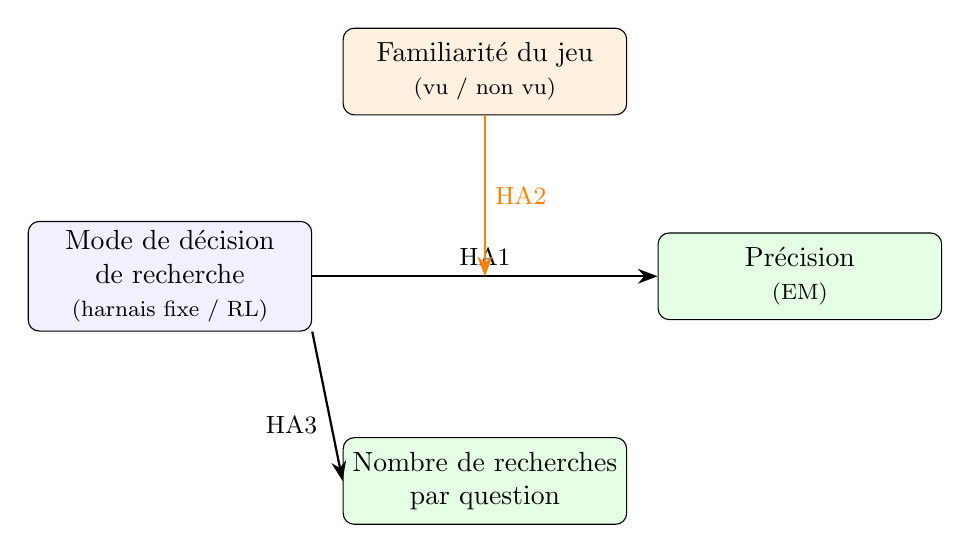
\begin{tikzpicture}[
  box/.style={draw, rounded corners, minimum width=3.6cm, minimum height=1.1cm, align=center, fill=blue!6},
  dep/.style={box, fill=green!10},
  mod/.style={box, fill=orange!12},
  >={Stealth[length=2.5mm]}]
  \node[box] (mode) at (0,0) {Mode de décision\\ de recherche\\ {\footnotesize (harnais fixe / RL)}};
  \node[dep] (em) at (8,0) {Précision\\ {\footnotesize (EM)}};
  \node[mod] (fam) at (4,2.6) {Familiarité du jeu\\ {\footnotesize (vu / non vu)}};
  \node[dep] (nb) at (4,-2.6) {Nombre de recherches\\ par question};
  \draw[->, thick] (mode) -- node[above, font=\small] {HA1} (em);
  \draw[->, thick, orange] (fam) -- node[right, font=\small] {HA2} ($(mode.east)!0.5!(em.west)$);
  \draw[->, thick] (mode.south east) -- node[below left, font=\small] {HA3} (nb.west);
\end{tikzpicture}
\caption{Modèle conceptuel. Lecture : le mode de décision influence la précision (HA1) ; cet effet dépend de la familiarité du jeu (HA2, flèche orange qui pointe sur la flèche HA1) ; le mode influence aussi le nombre de recherches (HA3).}
\label{fig:modele}
\end{figure}

\subsection{Hypothèses}
Nous numérotons les hypothèses de cet article HA1 à HA3. HA2 correspond à l'hypothèse H1 du mémoire, HA3 à son hypothèse H2.

\paragraph{HA1 (effet).} À corpus, retriever et questions identiques, les agents entraînés par renforcement (A4, A5) obtiennent une précision supérieure à celle des harnais fixes (A1 à A3).
\emph{Justification.} Le cadre de Simon suggère qu'une règle d'arrêt apprise sur la récompense s'ajuste mieux à la difficulté des questions qu'une règle fixée à l'avance. Les auteurs de Search-R1 rapportent des gains sur diverses lignes de base RAG \citep{jin2025search}, mais avec leurs propres lignes de base : HA1 est donc à tester, non à supposer.

\paragraph{HA2 (modération).} Cet avantage est plus fort sur le jeu vu à l'entraînement (Natural Questions) que sur le jeu non vu (TriviaQA).
\emph{Justification.} Les agents A4 et A5 ont été entraînés sur NQ et HotpotQA \citep{jin2025search}. Un gain mesuré sur NQ peut donc refléter une adaptation au jeu et non une meilleure décision de chercher.

\paragraph{HA3 (mécanisme).} Les agents entraînés par renforcement recherchent plus souvent que le harnais ReAct (A2), qui laisse le modèle décider : nombre moyen de recherches par question plus élevé, et recherche déclenchée même sur les questions auxquelles A0 répond juste.
\emph{Justification.} Sans coût dans la récompense, le cadre de Stigler prédit une surrecherche (section~\ref{sec:cadre}). Les travaux qui mesurent la surrecherche ou cherchent à réduire les appels \citep{wu2025search,tang2026saas,wang2025acting,zhao2025parallelsearch,mei2025ai,lin2025adasearch} suggèrent que le phénomène existe. À titre exploratoire, un test de la chaîne sur 20 questions de NQ, avec un sous-corpus de 100\,000 passages, donnait en moyenne 3,25 recherches par question pour A4 : ce chiffre n'a pas valeur de résultat.

\paragraph{Mesure.} Chaque concept correspond à une colonne des fichiers de résultats (tableau~\ref{tab:var}).
\begin{table}[ht]
\centering\small
\begin{tabular}{@{}lll@{}}
\toprule
Concept & Variable & Colonne\\
\midrule
Mode de décision & explicative & \texttt{system} (A0 à A5)\\
Familiarité du jeu & modérateur & \texttt{dataset} (\texttt{nq} ou \texttt{triviaqa})\\
Précision & expliquée & \texttt{em} (0 ou 1), \texttt{f1}\\
Nombre de recherches & expliquée (coût) & \texttt{n\_search}\\
\bottomrule
\end{tabular}
\caption{Variables du modèle et colonnes qui les mesurent.}
\label{tab:var}
\end{table}

\section{Méthode}\label{sec:methode}

\subsection{Systèmes}
Six systèmes sont comparés (tableau~\ref{tab:sys}). A0 à A3 utilisent le même modèle, Qwen2.5-3B-Instruct \citep{qwen2024qwen2}, avec des prompts écrits pour le projet ; A4 et A5 sont les points de contrôle publics de Search-R1 pour Qwen2.5-3B (versions 0.3, entraînés par PPO et par GRPO) \citep{jin2025search}. Les fichiers de configuration de ces points de contrôle indiquent qu'ils partent de Qwen2.5-3B, le modèle de base, et non de sa version Instruct. Les modèles de A0 à A3 et de A4/A5 diffèrent donc : un harnais par prompt demande un modèle qui suit des consignes, d'où ce choix, qui reste une limite discutée en section~\ref{sec:discussion}. Les systèmes disposent du même budget : au plus quatre recherches par question, trois passages par recherche, décodage glouton.

\begin{table}[ht]
\centering\small
\begin{tabular}{@{}llp{8cm}@{}}
\toprule
Code & Système & Règle de recherche\\
\midrule
A0 & Réponse directe & Aucune recherche\\
A1 & RAG & Une recherche avec la question\\
A2 & ReAct par prompt & Le modèle alterne Pensée, Action (\texttt{Search} ou \texttt{Finish}), Observation\\
A3 & IRCoT & Recherche avec la question, puis une recherche par phrase de raisonnement\\
A4 & Search-R1, PPO & Politique apprise par PPO\\
A5 & Search-R1, GRPO & Politique apprise par GRPO\\
\bottomrule
\end{tabular}
\caption{Les six systèmes.}
\label{tab:sys}
\end{table}

\subsection{Données et corpus}
Les questions viennent de Natural Questions \citep{kwiatkowski2019natural}, vu à l'entraînement de A4 et A5, et de TriviaQA \citep{joshi2017triviaqa}, non vu, dans le format de FlashRAG \citep{jin2024flashrag}. Nous tirons 100 questions par jeu avec la graine 42. Le corpus est un sous-ensemble d'un million de passages de l'instantané Wikipédia utilisé par Search-R1 ; le retriever est E5 \citep{wang2022text}, celui de l'entraînement de Search-R1.

Le sous-corpus n'est qu'une petite partie du corpus complet, ce qui limite ce que n'importe quel système peut retrouver. Nous avons mesuré, pour chaque jeu, la part des questions dont une réponse attendue apparaît parmi les trois premiers passages renvoyés avec la question pour requête. Avec E5 sur un million de passages, cette part est de 25~\% pour NQ et de 44~\% pour TriviaQA (500 questions par jeu) ; avec BM25 \citep{robertson2009probabilistic} sur 100\,000 passages, elle tombait à 9~\% et 12~\%, ce qui rendait la comparaison peu interprétable. C'est pourquoi nous avons retenu NQ et TriviaQA, et non HotpotQA et Bamboogle, dont la couverture est de 17~\% et 10~\% avec E5 sur un million de passages. Cette mesure est une estimation haute, car un passage peut contenir la réponse sans rapport avec la question.

\subsection{Mesures et statistiques}
La précision est la correspondance exacte (EM) et le score F1, avec la normalisation de Search-R1. Le coût est le nombre de recherches par question et le nombre de jetons générés. Nous donnons des intervalles de confiance à 95~\% par bootstrap \citep{efron1979bootstrap} (1\,000 rééchantillonnages de questions) et comparons deux systèmes sur les mêmes questions par le test de McNemar \citep{mcnemar1947note}. HA2 est évaluée par la différence entre l'écart mesuré sur NQ et l'écart mesuré sur TriviaQA, avec un intervalle bootstrap. Avec 100 questions par jeu, les intervalles font environ $\pm 10$ points : seuls des écarts importants seront détectables.

\section{Résultats}\label{sec:resultats}
\aremplir{résultats des runs sur Kaggle : tableau EM/F1/recherches par système et par jeu (tableau~\ref{tab:res}), figure EM selon le système, tests HA1 à HA3. Ne rien écrire avant d'avoir les fichiers JSONL.}

\begin{table}[ht]
\centering\small
\begin{tabular}{@{}lcccccc@{}}
\toprule
& \multicolumn{3}{c}{NQ (vu)} & \multicolumn{3}{c}{TriviaQA (non vu)}\\
\cmidrule(lr){2-4}\cmidrule(lr){5-7}
Système & EM & F1 & Rech. & EM & F1 & Rech.\\
\midrule
A0 & \aremplir{} & & & & &\\
A1 & & & & & &\\
A2 & & & & & &\\
A3 & & & & & &\\
A4 & & & & & &\\
A5 & & & & & &\\
\bottomrule
\end{tabular}
\caption{EM, F1 et nombre moyen de recherches par question (100 questions par jeu). Valeurs à insérer.}
\label{tab:res}
\end{table}

\section{Discussion}\label{sec:discussion}

\subsection{Rappel des résultats}
\aremplir{deux ou trois phrases : la réponse à la question de recherche, sans le détail des chiffres}

\subsection{Comparaison avec la littérature}
\aremplir{nos résultats confirment-ils, nuancent-ils ou contredisent-ils \citet{jin2025search} et les études de la section~\ref{sec:revue} ?}

\subsection{Explication}
\aremplir{retour au cadre de Stigler et Simon, surtout pour les résultats inattendus}

\subsection{Contributions}
\textbf{Théorique.} \aremplir{ce que l'étude apprend sur la décision de chercher}
\textbf{Pratique.} \aremplir{ce qu'un étudiant ou une équipe disposant d'un GPU gratuit peut en faire}

\subsection{Limites et pistes}
Ces limites valent quels que soient les résultats.
\begin{itemize}
  \item \textbf{Échantillon.} 100 questions par jeu, une seule graine, des intervalles d'environ $\pm 10$ points.
  \item \textbf{Corpus.} Un million de passages, avec une couverture de 25~\% (NQ) et 44~\% (TriviaQA) pour la réponse dans les trois premiers passages. Le plafond de précision d'un système qui dépend de la recherche est donc bas, et A4 et A5 ont été entraînés avec le corpus complet.
  \item \textbf{Modèles.} A0 à A3 utilisent Qwen2.5-3B-Instruct, A4 et A5 un modèle entraîné par renforcement à partir de Qwen2.5-3B (base) : l'écart observé mélange la règle de recherche et le modèle. Des points de contrôle partant de la version Instruct existent : ils permettraient de réduire cet écart dans le mémoire.
  \item \textbf{Prompts.} Ceux de A2 et A3 sont écrits pour ce projet avec deux exemples ; d'autres prompts pourraient changer les résultats.
  \item \textbf{Causalité.} Nous comparons des systèmes ; nous ne pouvons pas attribuer un écart à un seul facteur.
  \item \textbf{Part de l'IA dans la démarche.} Le corpus bibliographique, le code des systèmes et une première version de ce texte ont été produits avec un assistant (Claude). Les références ont été vérifiées dans OpenAlex ; les articles n'ont pas été lus en entier ; les choix de protocole et l'interprétation sont ceux de l'auteur. Le détail figure dans le carnet de bord.
\end{itemize}
\textbf{Pistes.} Deux hypothèses du mémoire ne sont pas testées ici : une pénalité par recherche dans la récompense réduit-elle le nombre d'appels sans perte forte de précision (entraînement GRPO à petite échelle), et un changement de retriever dégrade-t-il plus les agents entraînés que les harnais fixes ? Une analyse qualitative des échecs sur des trajectoires annotées compléterait la mesure.

\section{Conclusion}
\aremplir{à écrire après les résultats : 4 à 6 phrases}

\bibliographystyle{plainnat}
\bibliography{refs}
\end{document}
